\chapter{Architettura del sistema}
\label{ch:architecture}
Il \textit{Progetto Velocity} è un sistema di Track\&Trace il cui scopo è il monitoraggio in near real time della logistica.
Al momento il sistema monolitico legacy gestisce tutto, il nuovo sistema (Velocity) lo soppianterà gradualmente, seguendo un approcio Brownfield.
In questo momento si stanno sviluppando i nuovi servizi e li si sta integrando con il vecchio sistema.

\section{Sistemi coinvolti}
\label{sec:architecture_entity}

\begin{figure}[H]
\centering
    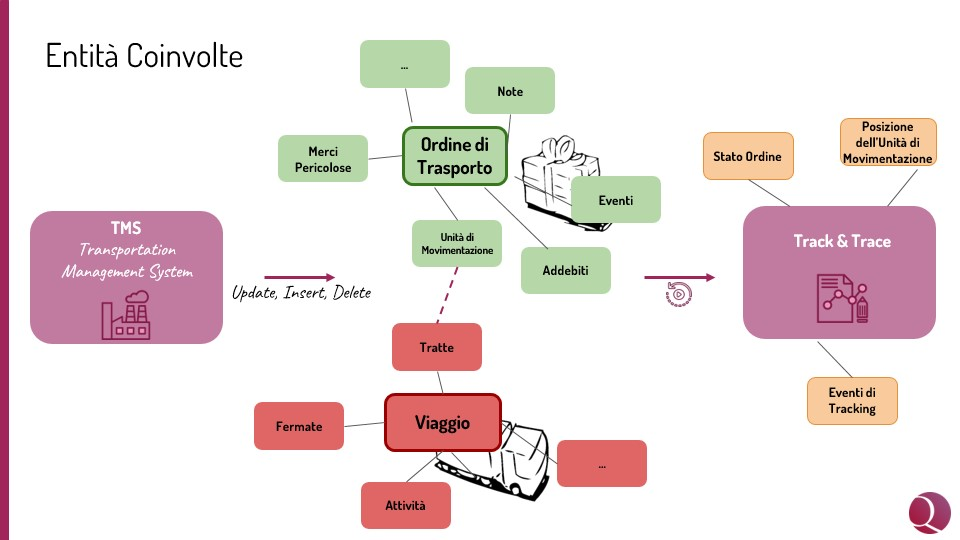
\includegraphics[scale=0.5]{images/architecture/entita_coinvolte.jpg}
    \caption{Entità coinvolte}
    \label{fig:architecture_entities_img}
\end{figure}

La sorgente dei dati è il \textit{Transport Management System (TMS)} un software esterno che effettua modifiche a diverse entità.
\todo{Queste entità logiche a livello pratico cosa sono} 
Le entità in questione sono raggruppabili diversi domini, i cui 3 principali sono:
\begin{itemize}
    \item Ritiro
    \item Ordine di trasporto (Spedizione)
    \item Viaggio
\end{itemize}
In figura \ref{fig:architecture_entities_img} sono presentati due domini d'esempio, \textit{Viaggio} e \textit{Ordine di Trasporto}.
\\
\\
I vari domini non sono isolati l'uno dall'alto, bensì la modifica di una entità potrebbe implicare la modifica di un'altra entità. In figura \ref{fig:architecture_entities_img} ad esempio modificando una \textit{unità di movimentazione} verrebbe conseguentemente modificata una \textit{tratta}.
\\
\\
Lo scopo del sistema di \textbf{T\&T} è proprio quello di tenere traccia di tutti i cambiamenti subiti dalle varie entità (effettuati dal \textbf{TMS}).
Ciò avviene tramite \texttt{Dbezium}\ref{sec:debezium_overview} che monitora i database del \textbf{TMS} generando eventi di dominio, che verranno poi processati da altri microservizi
%nel video quello che io chiamo entità vengono chiamati "root aggregate", anzi ancora diverso. sono tutte entità, ma le entità "viaggio" o "ordine trasporto" sono dei Root Aggregate, cioè degli oggetti che si portano dietro molte altre informazioni.
Il \textbf{T\&T} si occupa anche di fornire ai clienti informazioni sullo stato e sulla storia di diversi oggetti, composti dalle entità.
Ad esempio potrebbe essere fornito l'oggetto \textit{Carico} che descrive lo spostamento di un mezzo e tutte le consegne effettuate,
quindi costituito da \textit{Tratta e Fermate} ma anche dalle informazioni riguardo alle merci che trasporta, cioè \textit{Note,Unità di movimentazione, etc ...}

\section{Track and Trace legacy}
\label{sec:T&T_old}
Sistema basato su Batch, a regolari intervalli di tempo il sistema va a vedere il nuovo stato delle entità ed aggiorna un suo database interno di oggetti composti.
\todo{chiedere più info}

\section{Progetto Velocity}
\label{sec:T&T_new}
Sistema \textit{Event Driven} basato su \texttt{Kafka Streams}. \ref{subsubsec:kafka_stream}
Quando una entità cambia stato la modifica viene registrata su un \texttt{Kafka Topic} e successivamente gli eventi sui Topic vengono analizzati o filtrati tramite \texttt{Kafka Stream}.
Possiamo distinguere 3 tipologie di \texttt{Kafka Topic}:
\begin{figure}[H]
    \centering
    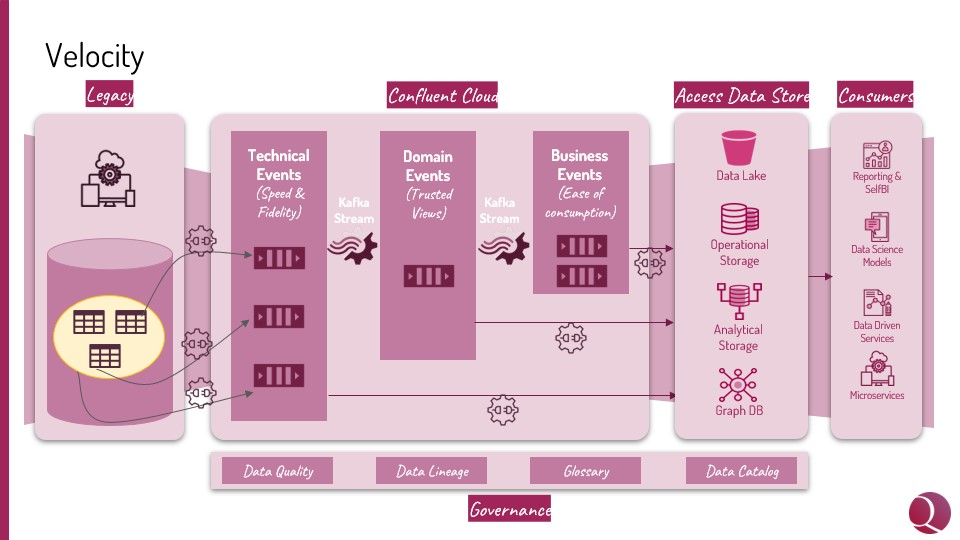
\includegraphics[scale=0.5]{images/architecture/confluent_velocity.jpg}
    \caption{Tipologie di Kafka Topics}
    \label{fig:kafka_topics.img}
\end{figure}
\begin{itemize}
    \item \textbf{Technical Events}: Contengono gli eventi generati dal \textbf{TMS}, sono eventi molto simili a dei log di un database
    (essendo generati tramite \texttt{Debezium} sono sostanzialmente una collezione di operazioni SQL) e spesso sono ridondanti, è
    infatti comune che il sistema effettui operazioni poco efficienti.
    Ad esempio qualora io avessi un ordine con una nota e la volessi modificare il TMS potrebbe svolgere la richiesta segnalando una operazione di \texttt{DELETE} ed una di \texttt{INSERT} piuttosto che effettuare una semplice \texttt{UPDATE}.\\
    É presente un \texttt{Topic} di tipo \textit{Technical Events} per ogni tabella del database originale (quindi un topic ogni dominio).
    \item \textbf{Domain Events}: Questi Topic contengono gli eventi filtrati dai \textit{Technical Events} tramite i \texttt{Kafka Streams}, non sono più simili a dei log di un DB (già solo la loro struttura è JSON, non SQL) e rappresentano come è fatto un oggetto (ordine di trasporto, viaggio, ...). 
    Tutti i potenziali eventi ridondanti sono stati filtrati dallo \textit{Stream}, non vi è più quindi il problema degli eventi ridondanti.
    \item \textbf{Business Events}: \texttt{Topic} opzionali, contengono degli eventi strutturati come i consumatori si aspettano (Ease of consumption). Sono pensati per fornire una vista specifica per un particolare consumer.
\end{itemize}

\subsection{Problema della consistenza}
\todo{farlo?}

\subsection{Componenti}
\label{subsec:components}

\subsubsection{Kafka Streams}
\label{subsubsec:kafka_stream}
\texttt{Kafka Streams} è una API per processare eventi su un \texttt{Topic Kafka} (filtrare, trasformare, aggregare, ...), questo tema viene approfondito nella sezione \ref{subsec:kafka_streams}\\
\\
Gli \texttt{Stream} che collegano i \texttt{Topic} di tipo \textit{Domain Events} a quelli di tipo \textit{Domain Business Event} sono molto dipendenti dalle necessità del consumatore che poi li leggerà quindi non seguono una struttura fissa, a differenza degli \texttt{Stream} che leggono dai \textit{Technical Events Topic} che svolgono operazioni suddivisibili in 3 fasi:
\begin{enumerate}
    \item \textbf{Fase di Casting}.\\
    In questa fase avviene la ricostruzione dell'evento basandosi sui log generati da \texttt{Dbezium} che sta osservando il \textbf{TMS}.\\
    Debezium si occupa di rilevare ogni cambiamento e pubblica l'evento su diversi topic kafka, uno per tabella (quindi uno per ogni dominio). 
    \item \textbf{Fase di Filtro}\\
    Successivamente gli eventi ridondanti devono essere eliminati. Tutti gli eventi relativi ad una transazione vengono accorpati e viene generato un unico evento risultante, che non riporta gli eventi intermedi. 
    \item \textbf{Fase di Mapping}\\
    Il nuovo evento viene quindi trasformato in un \textit{Domain Event} ed inserito sul relativo Topic.
\end{enumerate}

\subsubsection{MicroBatch}
\label{subsubsec:micro_batch}
Questo microservizio si occupa di "ricostruire" una entità a partire da tutti gli eventi che la riguardano. 
Non legge direttamente dal Topic \textit{Domain Events} quindi non è un \textit{consumer Kafka} bensì legge gli eventi di dominio da elaborare da un database SQL chiamato \texttt{Fast Storage} che viene continuamente aggiornato da un connettore JDBC di tipo Sink.
Gli eventi che riceve in input sono quindi dei \textit{Domain Events}, già filtrati dal relativo \texttt{Kakfa Stream}.\\
Dopo la "ricostruzione" l'oggetto viene riscritto nel Fast Storage, eliminando da esso gli eventi che lo riguardavano e che non sono più necessari.
Il microservizio \texttt{MicroBatch} è scritto usando \textit{Spring Batch} e lo scheduler su cui si appoggia per eseguire i Job è \textit{Quartz}.\\\\
Il primo passo, svolto ogni 5 secondi, è un partizionamento. Una classe \texttt{Spring Batch} chiamata \textit{Partitioner} divide gli eventi di dominio in \textit{chunks}, in modo da poterli processare in parallelo.
Il numero di \textit{chunks} è liberamente configurabile, ma il partizionatore è scritto in modo da raggruppare gli eventi con la stessa chiave di dominio (cioè relativi alla stessa Transazione) nella stessa partizione.
Questo non garantisce però che all'interno di un \textit{chunk} ci siano \textbf{solo} eventi con la stessa chiave di dominio.
A questo punto vengono eseguiti i vari \textit{Jobs}, uno per ogni \textit{chunk}, la cui esecuzione si può suddividere in 3 passi.
\begin{enumerate}
    \item \textbf{Reading}: Durante la fase di \textit{Reading} vengono recuperati dal Fast Storage tutti gli Eventi di Dominio che sono stati assegnati dal Partizionatore a quello specifico \textit{chunk}.
    \item \textbf{Processing}: Fase in cui si trasformano gli Eventi di Dominio recuperati durante la fase di \textit{Reading} in una serie di record pronti alla scrittura, ovvero in una serie di oggetti di tipo \texttt{Entity}.
    Le \textit{Entità} andranno quindi a comporre degli oggetti di vario tipo, infatti \texttt{MicroBatch} non si occupa di tenere aggiornata una sola tabella, bensì diverse tabelle sullo stesso database. \todo{quando avro accesso al DB potrò inserire questi esempi}
    Quindi partendo dagli stessi Eventi di Dominio verranno generati diversi record (diverse \texttt{Entity}) che verranno scritti su diverse tabelle.
    \item Writing:Fase finale di scrittura sul Fast Storage. É una scrittura transazionale, quindi deve rispettare le proprietà \texttt{ACID}, requisito di cui si occupa il \textit{Job}.
    Inoltre il \textit{Job} si occupa di verificare per ciascuna tabella se i dati che ha generato devono essere inseriti o solamente aggiornati.
\end{enumerate}

\subsubsection{Event Engine}
\label{subsubsec:event_engine}
Similmente a \texttt{Micro Batch} \ref{subsubsec:micro_batch} l'\textit{Event Engine} si occupa di "costruire" degli oggetti di business partendo dal \textit{Fast Storage}, questi oggetti sono pensati per la \textit{ease of consumption} di eventuali client.\\
In altre parole si occupa di osservare i cambiamenti di stato dei diversi eventi di dominio (segnalati dall \textbf{SGA} che monitora il \textbf{TMS}) e generare una serie di eventi di business associati (es: 
“spedizione partita”, “ritiro fallito”, “tempo di arrivo stimato”, …)\\\\
Rispetto al caso \texttt{Micro Batch} \ref{subsubsec:micro_batch}la fase di \textit{Reading} ritorna solo un record per ogni chiave di dominio, quindi ad ogni chunk corrisponde una e solo una chiave di dominio.
Invece le tre altre due fasi (\textit{Processing e Writing}) sono sostanzialmente identiche, con la differenza che la fase di Processing non va a generare un oggetto, bensì calcola una serie di metriche come "orario di partenza", "Tragitto", "Stato dell'ordine", etc ....